\documentclass[border=7pt]{standalone}

\usepackage{amsmath}  % Math fonts
\usepackage{amsfonts} %
\usepackage{amssymb}  %
\usepackage{tikz}
\usepackage{tkz-euclide}

\begin{document}

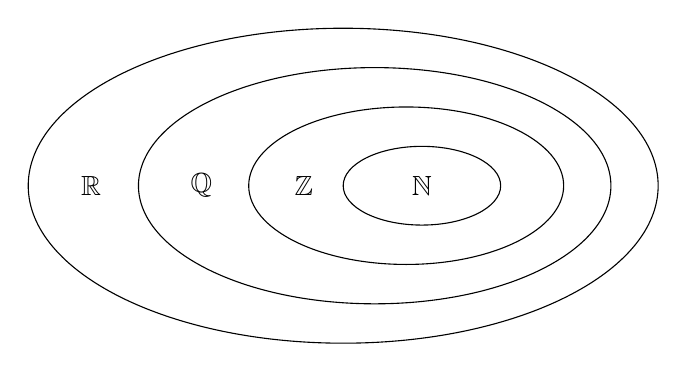
\begin{tikzpicture}
\filldraw[black] (-3.2,0) node {$\mathbb{R}$};
\filldraw[black] (-1.8,0) node {$\mathbb{Q}$};
\filldraw[black] (-0.5,0) node {$\mathbb{Z}$};
\filldraw[black] (1,0) node {$\mathbb{N}$};
\draw (0,0) ellipse (4cm and 2cm);
\draw (0.4,0) ellipse (3cm and 1.5cm);
\draw (0.8,0) ellipse (2cm and 1cm);
\draw (1,0) circle (1cm and 0.5cm);
\end{tikzpicture}

\end{document}
